\section{Hadronic Cross Section and Inverse Mellin}
We have managed to bring the partonic function on an exponentiated form, but the correct observable is the hadronic cross section. So in this section we will recover the hadronic Drell-Yan cross section in $x$-space, and discuss how the inverse Mellin transform can be evaluated. 

From \cref{eq:hadronic cross section in Mellin} and \cref{eq:LL result} the Mellin transformed hadronic cross section is given by
\begin{align}
    \tilde{\sigma}_{h_1h_2}(N)&=\int_{0}^{1}d\tau \tau^{N-1}\,\frac{1}{\sigma_{0}}\frac{d\sigma_{h_1h_2}}{dQ^{2}}\nonumber
    \\
    &=\sum_{i,j=q,\bar{q}}\tilde{f}_{i/h_1}(N,Q)\tilde{f}_{j/h_2}(N,Q)\,\exp\big(\Me{E}_{ij}(N,Q,\alpha_s)\big)\,,
\end{align}
where the partonic function has been exponentiated. We can now use the inverse Mellin transform \cref{eq:Appendix Inverse Mellin} to write\footnote{Where we have recovered the fractional charge of the quarks.}
\begin{align}
    \frac{d\sigma_{h_1h_2}}{dQ^{2}}=&\,\sigma_{0}\sum_{i,j=q,\bar{q}}Q_{q}^{2}\,
    \frac{1}{2\pi i}\int_{c-i\infty}^{c+i\infty}dN\,\tau^{-N}\tilde{f}_{i/h_1}(N,Q)\tilde{f}_{j/h_2}(N,Q)\exp\big(\Me{E}_{ij}(N,Q,\alpha_s)\big)\,.
\end{align}

There exists numerical packages to evaluate parton distributions in Mellin space, see \cite{Vogt_2005}. However, the standard method is to use parton distributions sets from the LHAPDF code existing is $x$-space \cite{whalley2005les,Buckley_2015}.  To use the $x$-space formalism we can do several manipulations by using the convolution properties of the Mellin transform, given in \cref{sec:Appendix Mellin Transform}. But let us first derive an expression for the inverse Mellin transform in terms of an integral over a real variable.

\subsection{The Inverse Mellin Transform}
The inverse Mellin transform for a general function is given in terms of an integral over a complex variable $N$, see \cref{sec:Appendix Mellin Transform}, and reads
\begin{align}\label{eq:h}
    h(x)=\frac{1}{2\pi i}\int_{c-i\infty}^{c+i\infty}dN\,x^{-N}\,\Me{h}(N)\,,
\end{align}
where 
\begin{align*}
    \Me{h}(N)=\int_{0}^{\infty}dx\,x^{N-1}\,h(x)\,.
\end{align*}
Since $h(x)$ is a real valued function
\begin{align}\label{eq:h_real}
    \Me{h}^{*}(N)=\int_{0}^{\infty}dx\,x^{N^{*}-1}\,h(x)=\Me{h}(N^{*})\,.
\end{align}

The Mellin inversion integral \cref{eq:h} can be splitt in two, one part for the lower bound and one part for the upper bound. To manipulate the integral, we make a change of variable $N\rightarrow N^{*}$ in the term that is integrated from $c-i\infty$ up to $c$. This makes the integration bound change accordingly $c-i\infty\rightarrow c+i\infty$, and we find
\begin{align}
    h(x)&=\frac{1}{2\pi i}\Bigl(\int_{c-i\infty}^{c}dN\,x^{-N}\,\Me{h}(N)+\int_{c}^{c+i\infty}dN\,x^{-N}\,\Me{h}(N)\Bigr)\nonumber
    \\
    &=\frac{1}{2\pi i}\Bigl(\int_{c+i\infty}^{c}dN^{*}\,x^{-N^{*}}\,\Me{h}(N^{*})+\int_{c}^{c+i\infty}dN\,x^{-N}\,\Me{h}(N)\Bigr)\nonumber
    \\
    &=\frac{1}{2\pi i}\Bigl(-\int_{c}^{c+i\infty}dN^{*}\,x^{-N^{*}}\,\Me{h}^{*}(N)+\int_{c}^{c+i\infty}dN\,x^{-N}\,\Me{h}(N)\Bigr)\,,
    \intertext{and by choosing the parametrization of the Mellin variable to be $N=c+ze^{i\phi}$, in terms of real $z$, the integral will take the form}
    h(x)&=\frac{1}{2\pi i}\int_{0}^{\infty}dz\,\left(e^{i\phi}\,x^{-N}\Me{h}(N)-e^{-i\phi}\,x^{-N^{*}}\Me{h}^{*}(N)\right)\nonumber
    \\
    &=\frac{1}{2\pi i}\int_{0}^{\infty}dz\,2i\,\text{Im}\left(e^{i\phi}\,x^{-N}\Me{h}(N)\right)\nonumber
    \\
    &=\frac{1}{\pi}\int_{0}^{\infty}dz\,\text{Im}\left(e^{i\phi}\,x^{-N}\Me{h}(N)\right)\,,
\end{align}
where we used \cref{eq:h_real} and the relation
\begin{align*}
    \Me{h}(N)-\Me{h}^{*}(N)&=2i\,\text{Im}(\Me{h}(N))\,.
\end{align*}

Writing out the parametrization, the final integral is given by
\begin{align}\label{eq:Inversed Mellin Integral}
    h(x)=\frac{1}{\pi}\int_{0}^{\infty}dz\,\text{Im}\left(e^{i\phi}\,x^{-c-z\,\exp(i\phi)}\Me{h}(c+z\,\exp(i\phi))\right)\,.
\end{align}


\subsection{Hadronic Cross Section in $x$-space}
In order to rewrite the inverse Mellin in $x$-space it is advantageous to use that \cref{eq:Factorized Dre-Yan Cross Section} is understood to be a Mellin convolution. Let us begin with \cref{eq:Factorized Dre-Yan Cross Section}, and use \cref{eq:Appendix Mellin convolution} to write it as\footnote{For simplicity we have abbreviated some of the arguments in the integrand.}
\begin{align}
    \frac{ d\sigma_{h_1h_2}}{dQ^{2}}=\sigma_{0}\sum_{i,j=q,\bar{q}}\int_{0}^{1}dz\,dx_{1}\,dx_{2}\,\delta\big(\tau-x_{1}x_{2}z\big) f_{i/h_1}(x_1)f_{j/h_2}(x_2)\,\omega_{ij}(z)\,,
\end{align}
and using the delta function property
\begin{align}\label{eq:delta_property}
    \int dx\,\delta(g(x))=\abs{\frac{\partial g}{\partial x}}_{x=x^{*}}^{-1}\int dx\,\delta(x-x^{*})\,,
\end{align}
we find that
\begin{align}\label{eq:rewritten convolution to inverse}
    \frac{ d\sigma_{h_1h_2}}{dQ^{2}}=\sigma_{0}\sum_{i,j=q,\bar{q}}\int_{\tau}^{1}\frac{dz}{z}\int_{\tau/z}^{1}\frac{dx_1}{x_1}f_{i/h_1}(x_1)f_{j/h_2}\Big(\frac{\tau}{x_1z}\Big)\,\omega_{ij}(z)\,,
\end{align}
where the limits have changed after acting with the delta function, i.e. we have
\begin{align}
    x_{2}=\frac{\tau}{x_1z}\leq 1\,,
    \hspace{0.7cm}
    \frac{\tau}{z}\leq x_1\leq 1\,,
    \hspace{0.7cm}
    \tau\leq z\leq 1\,.
\end{align}

%Then by Parseval's convolution theorem for the inverse Mellin transform, we have that
%\begin{align}
%    \int_{\tau}^{1}\frac{dz}{z}\int_{\tau/z}^{1}\frac{dx_1}{x_1}f_{i/h_1}(x_1)f_{j/h_2}\Big(\frac{\tau}{x_1z}\Big)\,\omega_{ij}(z)=\frac{1}{2\pi i}\int_{c-i\infty}^{c+i\infty}dN\,\tau^{-N}\tilde{f}_{i/h_1}(N)\tilde{f}_{j/h_2}(N)\Me{\omega}_{ij}(N)\,,
%\end{align}
%where it follows that we can evaluate the left hand side with $x$-space parton distributions, while $\omega(z)$ is evaluated as an inverse Mellin.

To actually perform the inverse transform is a nontrivial exercise, so let us go through some of the general details. The difficulty originates from the singularity structure of the integrand. These singularities can be divided into two regions in the complex $N$-plane, see \cref{fig:MP contour}. The first ones are positioned in the left part of the complex plane. These are the result of poles in the parton distribution functions $\Me{f}_{i/h}$. In general, the functional form of parton distributions functions at the initial scale $\mu_{0}$ is given by
\begin{align}
    xf_{i/h}(x,\mu_{0})=\sum_{n}A_{n}x^{\gamma_n}(1-x)^{\delta_n}\,,
\end{align}
where $A_{n}$, $\gamma_n$ and $\delta_{n}$ are obtained from a fitting procedure to hard scattering data, and for small $x$ and $\gamma_n<0$ this becomes singular. In Mellin space, this is transformed to
\begin{align}
    \Me{f}_{i/h}(N,\mu_{0})=\sum_{n}A_{n}\beta(N+\gamma_n,1+\delta_n)\,,
\end{align}
where $\beta(a,b)$ is the Euler-beta function in which the singular behaviour is well known. This first region can be avoided by choosing the contour in \cref{fig:MP contour}, as derived in \cite{Catani:1996}. We observe that the singularities from the parton distributions are avoided by choosing a constant $C_{MP}$ that lies to the right of the rightmost singularity of $\Me{f}_{i/h}$. 

The second region is more troublesome, as it is in the right part of the complex $N$-plane. This singularity originates from the Landau pole that arises for small couplings, i.e. the non-perturbative regime of QCD. The Landau pole manifest itself in the exponent of \cref{eq:LL result}, and is due to the expression $\ln(1-2\bar{\lambda})$. Hence, for $\bar{\lambda}=1/2$ we have
\begin{align}
    N_{L}=e^{-\gamma_{E}}e^{\frac{1}{2b_{0}\alpha_s}}\,.
\end{align}

This problem has been extensively studied in the litterature, and the most common approach is the so-called \emph{Minimal Prescription} \cite{Catani:1996}. This method states that the contour has to be chosen such that the constant $C_{MP}$, satisfies
\begin{align}
    C_{f}<C_{MP}<N_{L}\,,
\end{align}
where $C_{f}$ is the rightmost pole of $\Me{f}_{i/h}$. In \cref{fig:MP contour} we see the possible contours, where $C_{0}$ is the vertical line and $C_{1}$ is the bent contour. As argued in \cite{Catani:1996}, the choice $C_{MP}=2$ and $C_1$ with $\phi >\pi/2$, will make the integral converge faster than the choice $C_{MP}=2$ and $C_{0}$ with $\phi=\pi/2$.
\begin{figure}
    \centering
    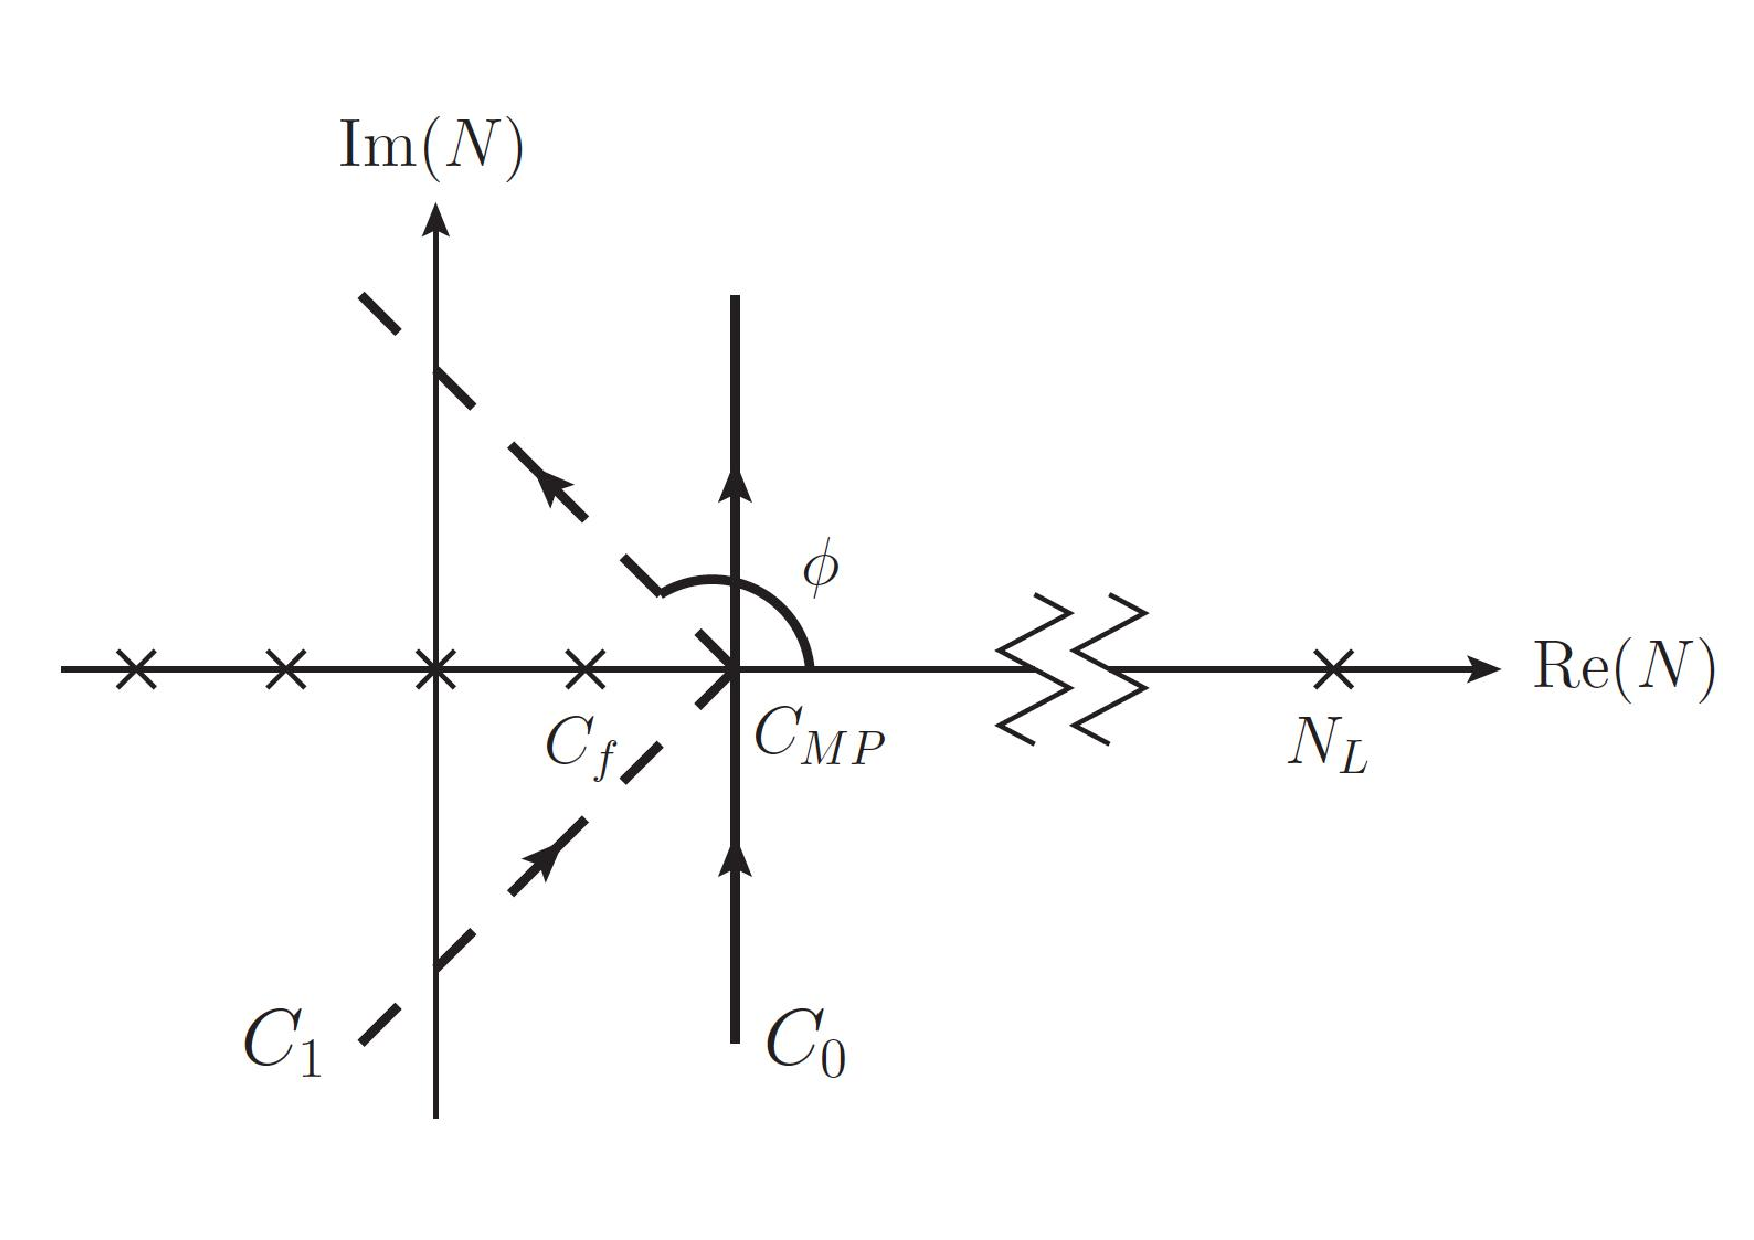
\includegraphics[scale=0.4]{Figures/CMP.pdf}
    \caption{Possibilities to choose the contour for the Mellin inversion as proposed in \cite{Catani:1996}. $C_{0}$ is the vertical contour and $C_{1}$ is the contour with an angle.}
    \label{fig:MP contour}
\end{figure}

So if the hadronic cross section is to be calculated with parton distributions in Mellin space, the following integral must be implemented
\begin{align}
    \frac{d\sigma_{h_1h_2}}{dQ^{2}}=&\,\sigma_{0}\sum_{i,j=q,\bar{q}}Q_{q}^{2}\,\frac{1}{\pi}\int_{0}^{\infty}dy\,\text{Im}\Big[e^{i\phi}\tau^{-N}\tilde{f}_{i/h_1}(N,Q)\tilde{f}_{j/h_2}(N,Q)\,\Me{\omega}_{ij}(N,\alpha_{s}(Q))\Big]\,,
\end{align}
where we used \cref{eq:Inversed Mellin Integral} to write the cross section as an integral over a real variable and $N=C_{MP}+ye^{i\phi}$. 

However, to use the $x$-space formalism the hadronic cross section is obtained by calculating
\begin{align}\label{eq:next to final hadronic}
    \frac{ d\sigma_{h_1h_2}}{dQ^{2}}=\sigma_{0}\sum_{i,j=q,\bar{q}}Q_{q}^{2}\int_{\tau}^{\infty}\frac{dz}{z}\int_{\tau/z}^{1}\frac{dx_1}{x_1}f_{i/h_1}(x_1,Q)f_{j/h_2}\Big(\frac{\tau}{x_1z},Q\Big)\,\omega_{ij}(z,Q,\alpha_{s}(Q))\,,
\end{align}
where the parton distributions are calculated in $x$-space, while the hard function is found by the inverse transform
\begin{align}
    \omega_{ij}(z,Q,\alpha_{s}(Q))=\frac{1}{\pi}\int_{0}^{\infty}dy\,\text{Im}\big(e^{i\phi}z^{-N}\,\Me{\omega}_{ij}(N,\alpha_{s}(Q))\big)\,.
\end{align}
We observe that the upper limit of the $z$ integral in \cref{eq:next to final hadronic} has changed. The reason for this change is that in the minimal prescription, the resummed cross section does not vanish for $z>1$ due to the Landau pole \cite{Catani:1996}. 

In \cref{eq:next to final hadronic}, the parton distributions are calculated in $x$-space, but there are problems that might occur in the hard function $\omega_{ij}$. Close to threshold, the resummed exponent can give large oscillations, see \cite{Catani:1996,KULESZA:2002} for more details. One possibility to dampen the oscillations is by a simple rewriting of the integrand. We do this by using \cref{eq:Appendix derivative of function}, to write
\begin{align}
    N\Me{f}_{i/h}(N)=\int_{0}^{1}dx\,x^{N-1}\mathcal{F}_{i/h}(x)\,,
\end{align}
where we used that parton distributions vanish for $x=1$, and defined
\begin{align}
    \mathcal{F}_{i/h}(x)=-x\frac{d}{dx}f_{i/h}(x)\,,
\end{align}
giving the modified hadronic cross section
\begin{align}
    \frac{ d\sigma_{h_1h_2}}{dQ^{2}}=\sigma_{0}\sum_{i,j=q,\bar{q}}Q_{q}^{2}\int_{\tau}^{1}\frac{dz}{z}\int_{\tau/z}^{1}\frac{dx_1}{x_1}\mathcal{F}_{i/h_1}(x_1,Q)\mathcal{F}_{j/h_2}\Big(\frac{\tau}{x_1z},Q\Big)\,\mathcal{S}_{ij}(z,Q,\alpha_{s}(Q))\,,
\end{align}
where
\begin{align}
    \mathcal{S}_{ij}(z,Q,\alpha_{s}(Q))=\frac{1}{2\pi i}\int_{C_{MP}}dN\,z^{-N}\frac{\Me{w}_{ij}(N,Q,\alpha_{s}(Q))}{N^{2}}\,.
\end{align}
The derivatives of the parton distributions can be performed numerically for the common sets \cite{Martin:2009,Pumplin:2002}. As mentioned the point of this rewriting is to dampen the behaviour of the exponent in $\omega_{q\bar{q}}$, but as argued in \cite{Catani:1996} gluon initiated processes should have even higher powers of $N$ as dampening factors. This would subsequently lead to higher order derivatives of the parton distributions.


 


